\documentclass{beamer}

% Top-aligning columns within a top-aligned frame
% https://tex.stackexchange.com/questions/16447/beamer-top-aligning-columns-within-a-top-aligned-frame
\makeatletter
\newenvironment{myitemize}{%
   \setlength{\topsep}{0pt}
   \setlength{\partopsep}{0pt}
   \renewcommand*{\@listi}{\leftmargin\leftmargini \parsep\z@ \topsep\z@ \itemsep\z@}
   \let\@listI\@listi
   \itemize
}{\enditemize}
\makeatother  

\usepackage[USenglish]{babel}
\usepackage[utf8]{inputenc}
\usepackage{amssymb, amsmath}
\usepackage{bm}
\usepackage{color}
\usepackage{tikz}
\usepackage{url}

\definecolor{links}{HTML}{2A1B81}
\hypersetup{colorlinks,linkcolor=,urlcolor=links}

\usetheme{Boadilla}
\setbeamertemplate{headline}{}
\newcommand*\oldmacro{}%
\let\oldmacro\insertshorttitle%
\renewcommand*\insertshorttitle{%
  \oldmacro\hfill%
  \insertframenumber\,/\,\inserttotalframenumber}
  

\bibliographystyle{apalike}
% make bibliography entries smaller
%\renewcommand\bibfont{\scriptsize}
% Now get rid of all the colours
\setbeamercolor*{bibliography entry title}{fg=black}
\setbeamercolor*{bibliography entry author}{fg=black}
\setbeamercolor*{bibliography entry location}{fg=black}
\setbeamercolor*{bibliography entry note}{fg=black}

\newcommand{\lnorm}[1]{\left\lVert#1\right\rVert^2}
\newcommand{\norm}[1]{\left\lVert#1\right\rVert}

% and kill the abominable icon
\setbeamertemplate{bibliography item}{}

\begin{document}
\title{Dropout is a special case of the stochastic delta rule: faster and more accurate
deep learning}  
\author{Radek Bartyzal}
\date{28. 2. 2019} 
\institute{Let's talk ML in Prague}

\frame{\titlepage} 

\begin{frame}{Dropout}

\begin{itemize}
\item add stochasticity = escape local minima
\item removes hidden units according to a Bernoulli
random variable with probability p prior to each
update

\item $\implies$ gradient updates affect non-removed neurons only
\item $\implies$ exponential number of networks averaged over updates
\item $\implies$ increase generalization by model averaging
\end{itemize}

\end{frame}

%--------- END Frame 1 -------------
\begin{frame}{Stochastic Delta Rule: Motivation}

\begin{itemize}
\item neural transmissions involve noise
\item neuron stimulated with same stimuli will never result in the same response
\item smooth neural rate
functions = averaging over many stimulation trials
\item $\implies$ synapse between two neurons could be modeled with a distribution with fixed parameters
\end{itemize}

\end{frame}
%--------- END Frame 1 -------------
\begin{frame}{Stochastic Delta Rule: Idea}

\begin{itemize}
\item each weight $w_{ij}$ = random variable with mean $\mu_{w_{ij}}$ and standard
deviation $\sigma_{w_{ij}}$
\item we assume Gaussian but can be other distr.
\item weight random variable is
sampled on each forward activation

\end{itemize}


\begin{figure}[h]
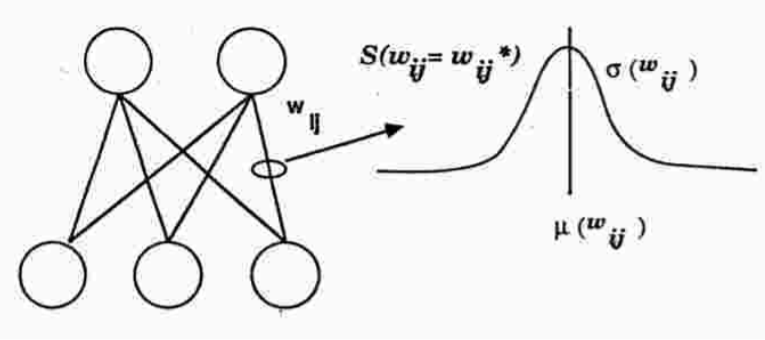
\includegraphics[width=0.8\textwidth]{img/sampling}
\end{figure}

\end{frame}
%--------- END Frame 1 -------------
\begin{frame}{Stochastic Delta Rule: Details}

\begin{itemize}
\item exponential number of potential networks with shared weights

\vfill

\item Both parameters are updated according to prediction error
\item $\implies$ weight noise injections reflecting local history of prediction error = bigger error $\implies$ bigger $\sigma$
\item $\implies$ local model averaging
\item model averaging may smooth out ravines in the
error surface [Hinton]

\vfill

\item simulated annealing per weight
\item each weight is updated based on its sampled contribution = gradient is a random variable

\end{itemize}

\end{frame}


%--------- END Frame 1 -------------
\begin{frame}{Stochastic Delta Rule: Update rules}

Forward pass samples weights $w^{*}_{ij}$ from $N(\mu_{w_{ij}},\sigma_{w_{ij}})$:
\begin{figure}[h]
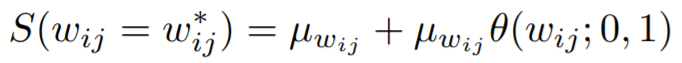
\includegraphics[width=0.6\textwidth]{img/init}
\end{figure}

Classic gradient update to mean:
\begin{figure}[h]
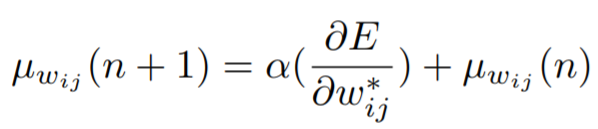
\includegraphics[width=0.5\textwidth]{img/update_mu}
\end{figure}

Bigger error $\implies$ bigger $\sigma$ = increase temperature:
\begin{figure}[h]
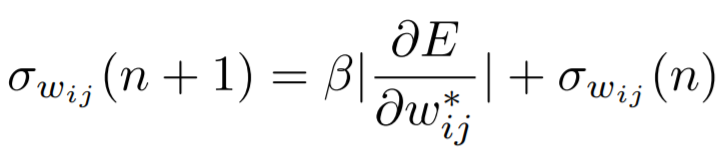
\includegraphics[width=0.5\textwidth]{img/update_sigma}
\end{figure}

Exponentially lower $\sigma$ = lower temperature = converge:
\begin{figure}[h]
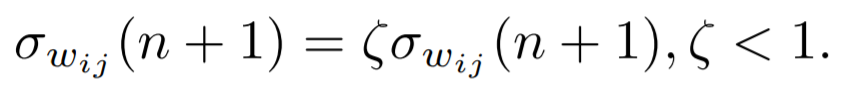
\includegraphics[width=0.5\textwidth]{img/update_sigma_2}
\end{figure}



\end{frame}
%--------- END Frame 1 -------------
\begin{frame}{Dropout is Stochastic Delta Rule}

\begin{itemize}
\item Bernoulli random variable over many trials results in a Binomial distribution with mean $np$ and standard deviation $(np(1-p))$. 
\item The random variable is the number of removals  over learning
\item Dropout = hidden unit Binomial sampling
\end{itemize}

\begin{figure}[h]
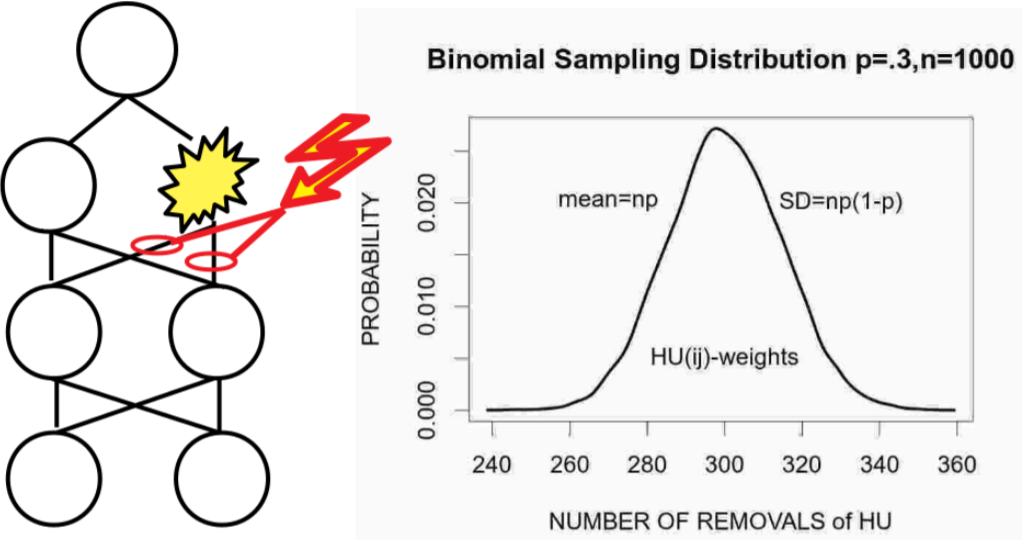
\includegraphics[width=0.7\textwidth]{img/dropout_sampling}
\end{figure}

\end{frame}
%--------- END Frame 1 -------------
\begin{frame}{Experiments}

\begin{itemize}
\item DenseNet-40, DenseNet-100, DenseNet-BC 250
\item original parameters kept 
\item dropout = 0.2
\item $\alpha$/LR dropping at 50\% and 75\% of the run
\item around $\alpha=0.25$, $\beta= 0.05$, $\gamma= 0.7$
\item annealed $\gamma$ to reduce the influence of  $\sigma$ as the model converges
\item $\sigma$ updated twice every epoch, in the middle and at the end, for DenseNet-BC 250 and DenseNet-100 and after every batch for the others
\item number of updates per epoch affects performance = new hyperparameter
\item earlier layers have $\gamma=0.9 * \gamma$
\end{itemize}

\end{frame}
%--------- END Frame 7 -------------
\begin{frame}{Results}
\begin{figure}[h]
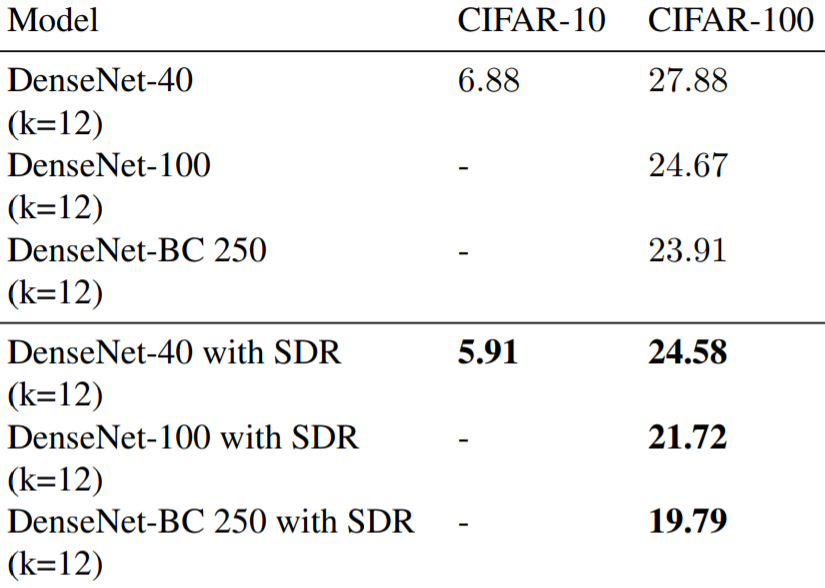
\includegraphics[width=0.9\textwidth]{img/results}
\end{figure}
\end{frame}
%--------- END Frame 7 -------------
\begin{frame}{Results}
\begin{figure}[h]
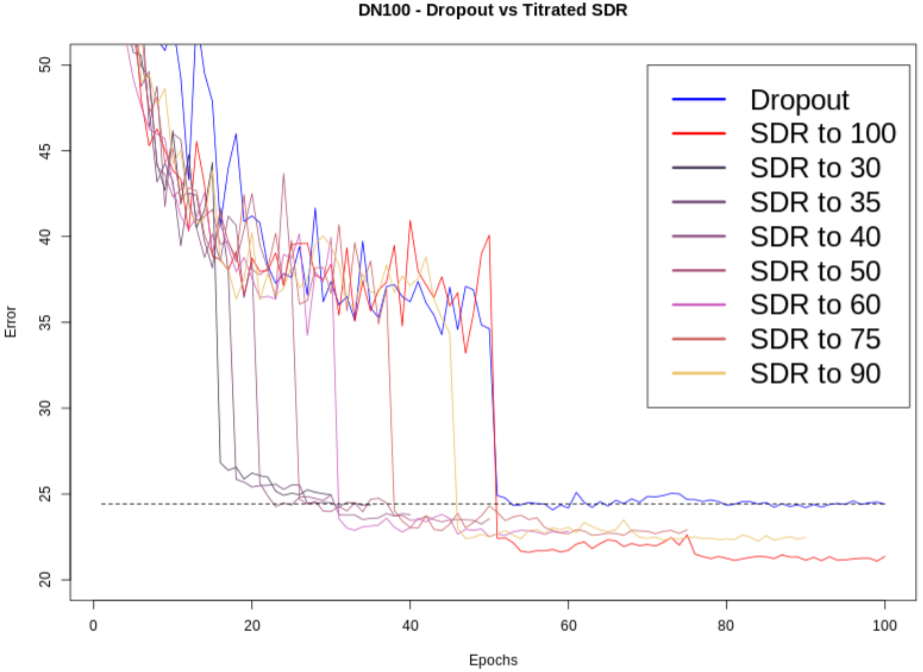
\includegraphics[width=0.9\textwidth]{img/titrated}
\end{figure}
\end{frame}
%--------- END Frame 7 -------------
\begin{frame}{Results}
\begin{figure}[h]
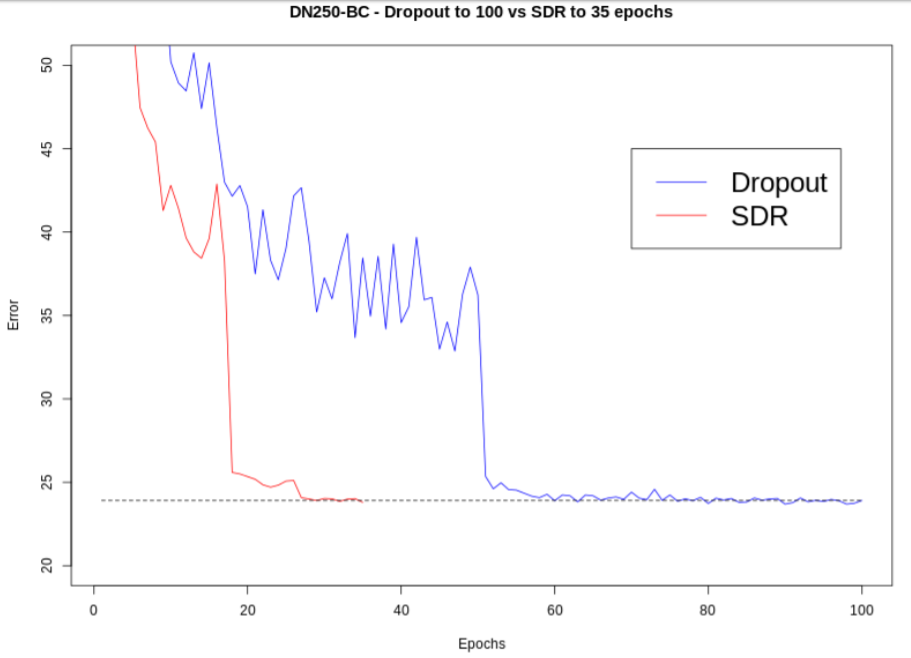
\includegraphics[width=0.9\textwidth]{img/dropout_vs_sdr}
\end{figure}
\end{frame}


%--------- END Frame 12 -------------
\begin{frame}{Sources}

\begin{thebibliography}{0}

  \bibitem[1]{cit:drop} 1. Frazier-Logue, Noah, and Stephen José Hanson. "Dropout is a special case of the stochastic delta rule: faster and more accurate deep learning." arXiv preprint arXiv:1808.03578 (2018). \url{https://arxiv.org/pdf/1808.03578v2.pdf}
  
\end{thebibliography}

\end{frame}

 
 
 
\end{document}
